\begin{frame}{BeepTrace}

    \centering
    BeepTrace proposes an alternative framework for contact tracing applications based on blockchain technology. The initiative is open and is still under development and testing.
    
    \begin{columns}[T]
        \column{0.3\linewidth}
        \begin{block}{Objectives}
            \begin{itemize}
                \item Transparency
                \item Immutability
                \item Security
                \item Privacy
            \end{itemize}
        \end{block}
        
        \column{0.6\linewidth}
        \begin{block}{Reference}
            \small{Xu, H., Zhang, L., Onireti, O., Fang, Y., Buchanan, W.B., \& Imran, M. (2020). BeepTrace: Blockchain-enabled Privacy-preserving Contact Tracing for COVID-19 Pandemic and Beyond. ArXiv, abs/2005.10103.}
        \end{block}
    \end{columns}
    
    \vspace{10pt}
    
    \centering
    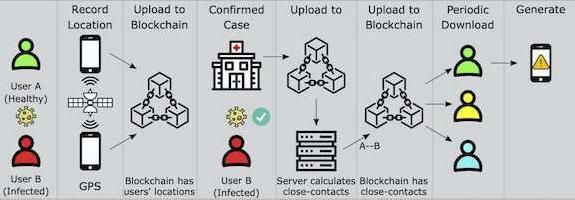
\includegraphics[width=0.8\linewidth]{images/beeptrace.jpg}
\end{frame}

\begin{frame}{BeepTrace}
    \begin{block}{Actors}
        \begin{description}[Pos. Providers]
            \item[Users] Each person using actively the application. 
            \item[Diagnosticians] GPs that verify whether the user is the rightful holder of pseudonyms and sign positive cases.
            \item[GeoSolvers] Servers which compute risks and update notifications for the users.
            \item[Authorities] Governments or other authorities which provide authorizations and keys.
            \item[Pos. Providers] GNSS, Bluetooth, Cellular Towers, and WiFi, used to certificate new users as well
        \end{description}
    \end{block}
    
    \begin{block}{Privacy}
        Privacy is guaranteed by design enabling only authorized entities to see the information strictly related to their duty.
    \end{block}
    
    \begin{block}{Blockchain}
        Solution based on two DLTs, the \textbf{notification} one and the \textbf{tracing} one.
        Consensus mechanism represents a crucial decision, they opted for a DAG-based solution. Contact tracing can be seen as a special case of Internet of Things.
    \end{block}
\end{frame}